\subsection{Setup}
\label{subsec:experimental_setup}

As already anticipated, material property modulation is achieved by means of shunted piezoelectric patches.
Figure \ref{fig:experimental_setup} illustrates the experimental setup, highlighting the placement of the piezoelectric patches and the shunt circuits.

\begin{figure}[H]
    \centering
    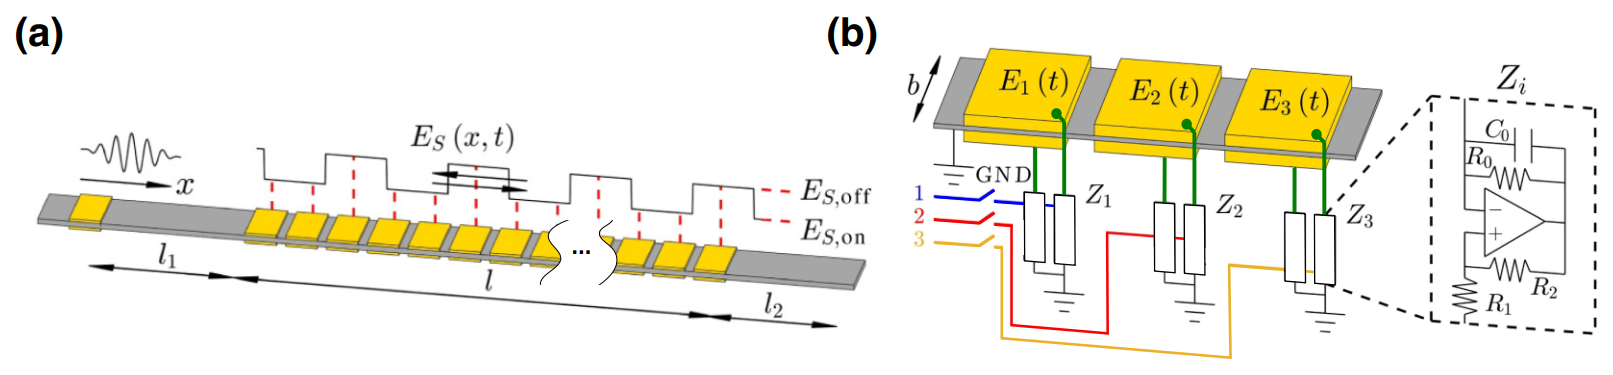
\includegraphics[width=0.9\textwidth]{./img/experimental_setup_scheme.png}
    \caption{Schematic of the experimental setup.}
    \label{fig:experimental_setup}
\end{figure}

In particular, Figure \ref{fig:experimental_setup} (a) depicts the electromechanical beam, including the excitation patch (responsible for generating the travelling wave signal) and the active domain containing the array of piezoelectric patches.
Figure \ref{fig:experimental_setup} (b) provides a close-up view of the unit spatiotemporal (ST) cell, consisting of three piezoelectric patches and the corresponding $C_N$ type shunt circuits.
Active modualtion is achieved by toggling switches that control the connection between the power supply and operational amplifiers.

The host beam consists of an aluminum substrate with a cross-section of $20 mm \times 1 mm$ and a total length of $2400 mm$.
An array of piezoelectric patches, spaced $2 mm$ apart, is positioned at $l_1 = 690 mm$ and $l_2 = 1134 mm$ from the beam's left and right boundaries, respectively.
This choice of placement minimizes boundary reflections, further mitigated by the use of absorbing boundary layers composed of mastic tape.

The active piezoelectric region, spanning $576 mm$, consists of $24$ pairs of piezoelectric patches with dimensions $20 mm \times 22 mm \times 1 mm$.
These patches are bonded on opposite surfaces of the beam and connected to a total of $48$ negative capacitance shunt circuits.
When the circuit is closed, the effective stiffness of the beam section is reduced (see Equation \ref{eq:weighted_average_mechanical_properties}).

The out-of-plane velocity field along the beam's length is measured using a Polytec 3D laser Doppler vibrometer (SLDV).

In Table \ref{tab:experimental_setup_parameters}, the main parameters of the experimental setup are summarized.

\begin{table}[H]

    \centering

    \begin{tabular}{|l|c|c|c|}
        \hline
        \textbf{Parameter}                 & \textbf{Symbol} & \textbf{Value} & \textbf{Units} \\
        \hline
        Beam Young's modulus               & $Y_b$           & $69$           & $GPa$          \\
        Beam density                       & $\rho_b$        & $2700$         & $kg/m^3$       \\
        \hline
        Piezoelectric Young's modulus      & $Y_1^E$         & $62$           & $GPa$          \\
        Piezoelectric capacitance          & $C_T$           & $7.0$          & $nF$           \\
        Piezoelectric coupling coefficient & $k_{31}$        & $0.351$        & -              \\
        Piezoelectric density              & $\rho$          & $7900$         & $kg/m^3$       \\
        \hline
        Shunt capacitance                  & $C_0$           & $4.4$          & $nF$           \\
        Shunt bias resistance              & $R_0$           & $1.0$          & $M\Omega$      \\
        Shunt resistance                   & $R_1$           & $7.5$          & $k\Omega$      \\
        Shunt resistance                   & $R_2$           & $13.7$         & $k\Omega$      \\
        \hline
    \end{tabular}

    \caption{Main parameters of the experimental setup.}
    \label{tab:experimental_setup_parameters}

\end{table}